\documentclass[prl,twocolumn,showpacs]{revtex4}

\usepackage{epsfig,color,graphicx,amsmath}
\begin{document}
\newcommand{\ltwid}{\mathrel{\raise.3ex\hbox{$<$\kern-.75em\lower1ex\hbox{$\sim$}}}}
\newcommand{\gtwid}{\mathrel{\raise.3ex\hbox{$>$\kern-.75em\lower1ex\hbox{$\sim$}}}}
\newcommand{\bra}{\langle}
\newcommand{\ket}{\rangle}
%\newcommand{\sill}{\psi_\mathrm{SILL}}
\newcommand{\sill}{\psi}
\newcommand{\trace}{{\rm Tr}}
\newcommand{\ntilde}{\tilde{n}}
\newcommand{\stilde}{\tilde{s}}
\newcommand{\atilde}{\tilde{\alpha}}
\newcommand{\new}{\color{red}}
\newcommand{\old}{\color{black}}
\newcommand{\bea}{\begin{eqnarray}}
\newcommand{\eea}{\end{eqnarray}}
\def\nn{\nonumber\\}

\bibliographystyle{apsrev}

\title{Establishing a fundamental connection between the covalent component of the
hydrogen bonding network and properties of liquid water}

\author{Yifei Shi}
\affiliation{Department of Chemistry, McGill University, 801 Sherbrooke St. West, Montreal, QC H3A 0B8, Canada}

\author{Hayden Scheiber}
\affiliation{Department of Chemistry, McGill University, 801 Sherbrooke St. West, Montreal, QC H3A 0B8, Canada}

\author{Rustam Khaliullin}
\affiliation{Department of Chemistry, McGill University, 801 Sherbrooke St. West, Montreal, QC H3A 0B8, Canada}

%\date{\today}

\begin{abstract}
Many remarkable properties of liquid water originate from the ability of water molecules to form hydrogen bond, which is a combination of electrostatic, induction, dispersion and covalent interactions. In this work, we developed an ab initio molecular dynamics method that enabled us to adjust the spatial extent of the covalent component of interactions between water molecules in simulations. We show that for room-temperature liquid water, a seemingly small amount of electron transfer has a profound effect on observable properties of liquid water. In particular, the tetrahedronal structure, O-H stretch mode and viscocity are all significantly determined by covalent interactions.


\end{abstract}
\maketitle

\section{Introduction} 

Detailed understanding of the physical nature of hydrogen bonding (HB) between molecules in water is essential to unravel origins of the unique properties of this ubiquitous and important liquid. It has been known since the dawn of quantum mechanics that hydrogen bonding is a complex phenomenon that arises from the interplay of several distinct effects: interaction between molecules’ permanent multipoles (dipoles, quadrupoles, etc.), polarization, dispersion, and donor-acceptor orbital interactions that lead to partial electron transfer between molecules. Recent developments in electronic structure methods have helped to make progress towards solving a long-standing problem of quantifying the individual contributions of these effects to the energy of hydrogen bonding. One last unresolved issue has been the extent of intermolecular charge transfer in hydrogen bonding \cite{isaacs1999covalency,ghanty2000hydrogen,stone2017natural}.
Natural bond orbital (NBO) analysis\cite{weinhold1998natural} and natural energy decomposition analysis \cite{glendening1994natural} suggest that charge transfer (CT) is predominant \cite{schenter1996natural,glendening2005natural,weinhold2005resonance} because, if charge transfer is neglected, NBO analysis shows no binding at the water-dimer equilibrium geometry. However, other earlier decomposition methods \cite{kitaura1976new,bagus1984new,bagus1992decomposition,stevens1987frozen,chen1996energy} as well as as most recently developed alternatives \cite{mo2000energy,misquitta2003dispersion,khaliullin2007unravelling} estimated that CT contributes only around 20\% of the overall binding energy. After a debate spanning several decades, it is becoming clear that NBO is not optimized to treat intermolecular interactions\cite{stone2017natural}, and covalent donor-acceptor component contributes only a small portion to the overall binding energy between water molecules in small clusters \cite{stevens1987frozen,chen1996energy,piquemal2005csov,khaliullin2009electron,cobar2012examination}.



The success of energy decomposition techniques allowed us to look beyond a simple contribution of charge transfer to the interaction energy and to establish a fundamental connection between physical components and the observed properties of water – an area, in which our knowledge remains rudimentary at best. In this work, we coupled ab initio molecular dynamics to a recently developed energy decomposition method for periodic systems \cite{Khaliullin2013JCTC} to perform an unprecedented computational study that enabled us to quantify the contribution of the covalent component of hydrogen bonding to the structural, dynamical and spectroscopic properties of liquid water at ambient conditions. We showed that even a seemingly insignificant covalent component of hydrogen bonding has a profound effect on the properties of water.


\section{Methods}

To isolate the effect of the covalent component of hydrogen bonding on the properties of liquid water, we performed ab initio molecular dynamics simulations using a special version of density functional theory based on absolutely localized molecular orbitals (ALMO)\cite{khaliullin2006efficient,Khaliullin2013JCTC}. In ALMO, each molecular orbital (MO) is expanded in terms of the atomic orbitals (AOs) of a fragment containing a certain number of molecules, thus the charge transfer between molecules can easily be adjusted by changing the number of molecules in the fragment. In this work each fragment will have only one molecule, totally excluding any intermolecular charge transfer. 
\new{what to say about ALMO MD?} \old


In order to compare properties of liquid water with and without charge transfer, we look at the system described by ALMO with zero charge transfer, and the system described by normal DFT. The former will be refered to as localized system and the latter delocalized or reference system. We use BLYP functional, TZV2P basis set, and D3 dispersion correction for both systems. The density of these systems are set to be 1g/cm$^3$(\new the densities of systems are slightly(within 5\%) different, but I thought it's not necessary to list all of them \old) for a MD simulation with NVT ensemble at a temperature of 298K with periodic boundary condition. Since properties like density or pressure can be affected by covalency, we also look at a third system whose density is determined by a NPT simulation at a constant pressure of 1atm. This system will be denoted by low density localized system.


\section{Results}

\textbf{Static properties} The Oxygen-Oxygen radial distribution function (RDF) is shown in Fig~\ref{Fig:RDF}. The position of the peak moved from 2.8$\mathring{\text{A}}$ to 3.1$\mathring{\text{A}}$. It is clear that the molecules in the localized system turns to be further away, since the interaction between molecules are weaker. \new The O-O peak seems to only depend on the interaction strength. Here the density is the same for both systems, but the molecules seem to get further away. While for the results shown in Fig~\ref{Fig:rdf_cp} the densities are different but the peaks are at the same position. How to interpret this? \old

\begin{figure}
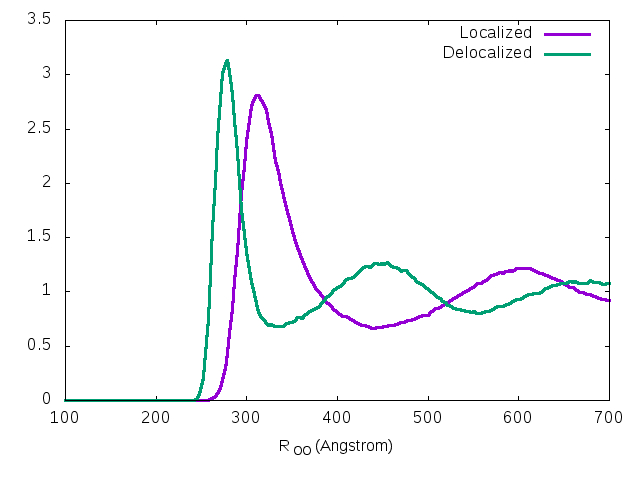
\includegraphics[width=0.4\textwidth]{RDF}
\caption{Oxygen-Oxygen radial distribution function for localized and delocalized water systems. The calculation was done for  125 water molecules with NVT ensemble. The average distance between molecules and the position of the first solvent shell are all larger for the localized system. \new Add O-H RDF? \old} \label{Fig:RDF}
\end{figure}


To understand how the directional feature of HBs depends on covalency, we look at the spacial distribution function of Oxygen atom, and the distribution of the H-O-O angle, shown in Fig~\ref{Fig:ADF}. For the delocalized water molecule, the HBs are strongly directional, favouring the tetrahedronal structure. Without covalency, the water molecules do remain directional, although the peak is much more diffused. The width of the peak increases from $\sim 10 ^{\circ}$ to $\sim 25^{\circ}$, indicating covalent interaction is a major factor in the orientation of water molecules. However, even without covalent interactions water molecule would remain directional. This is further illustrated in Fig~\ref{Fig:SDF}, where the spacial distribution function (SDF) of the Oxygen atom of 2 cross sections are shown. \new It's interesting to note that the oxygen atoms still prefer to stay around the position, indicating that electrostatic and polarization interactions tend to orient water molecules the same way as charge transfer interaction, although the effect is much weaker. \old

We also show in Tab~\ref{HBstat}, how many HBs a molecule donate(D) or accept(A), with a geometric criterion that the H-O-O angle is smaller than 30$^{\circ}$ and the O-O distance is smaller than 3.5$\mathring{\text{A}}$. The number of HBs is 35\% less in the localized system.

\begin{table}
\caption{HB statistics for localized and delocalized system.}\label{HBstat}
\begin{tabular}{l|*{5}{c}}
\hline
Num. of HBs              & 0 & 1 & 2 & 3 &mean HBs \\
\hline
Localized(D)               & 13.3\% & 46\% & 40.1\% & 0.5\% & 1.277  \\
Localized(A)               & 15.7\% & 46.4\% & 32.5\% & 5.2\% & 1.266 \\
Delocalized(D)             & 0.3\% & 9.9\% & 89.4\% & 0.4\% & 1.899\\
Delocalized(A)             & 0.4\% & 16.3\% & 76.3\% & 6.9\% & 1.896 \\

\end{tabular}

\end{table}


\begin{figure}
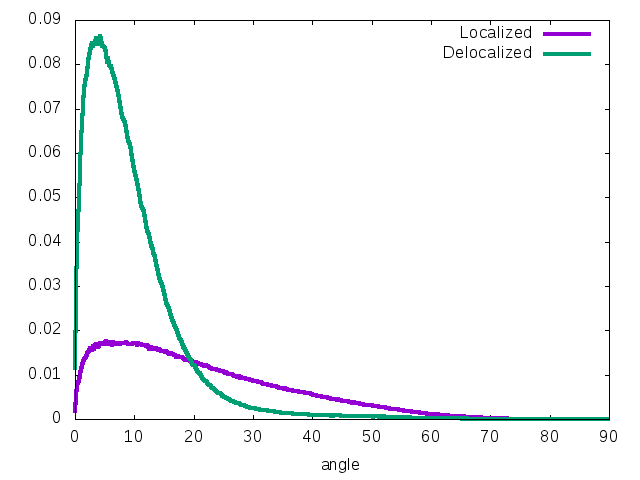
\includegraphics[width=0.4\textwidth]{angular_dist}
\caption{Angular distribution of the H-O-O angle, for delocalized and localized systems. The curves are normalized so that the total integral $\int g(\theta)2\pi \text{sin}(\theta)d\theta = 1$. \new All other plots I have seen use the other way to normalize \old} \label{Fig:ADF}
\end{figure}

\begin{figure}
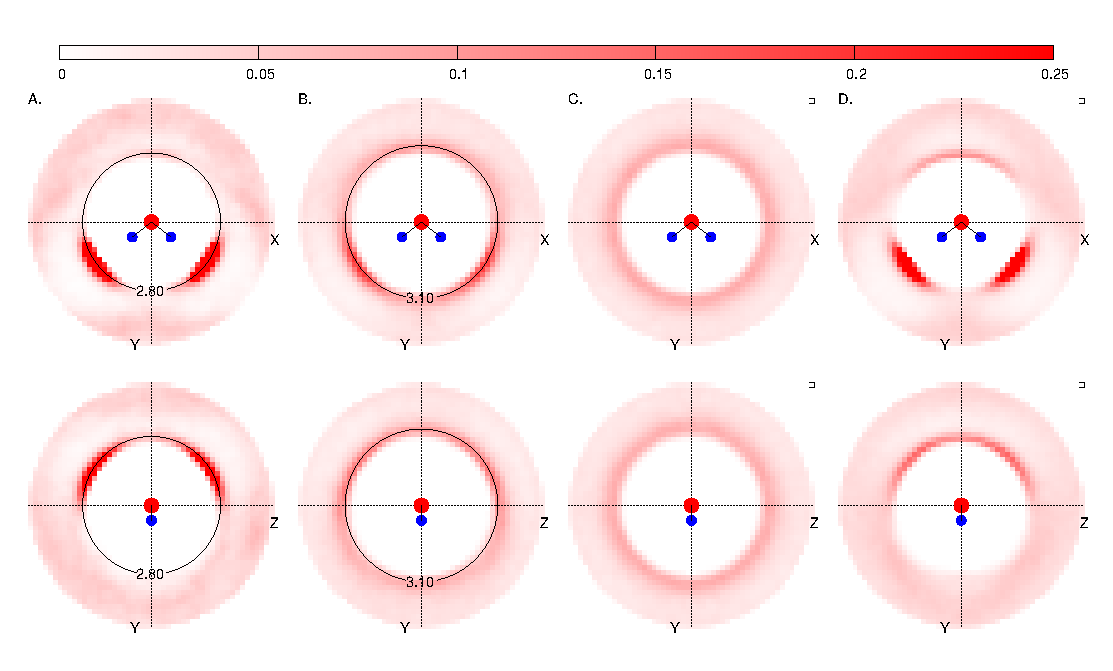
\includegraphics[width=0.45\textwidth]{SDF}
\caption{angular and spacial distribution. Cross sections of spacial distribution. The upper half shows the cross section of SDF in the plane parallel to the water molecule, and the lower half shows the cross section perpendicular to the molecule. (a) Delocalized reference system. (b) Localized system. The Oxygen atom still prefer to stay around the positions corresponding to the tetrahedronal structure. (c) Classical simulation with only Van der Waals force. This case the molecules are truely none-directional, and the angular distribution is uniform. (d) Classical simulation with charge and Van der Waals force. This case the water molecules retain the tetrahedronal structure. } \label{Fig:SDF}
\end{figure}

\textbf{HB life time}
The HB decay function $C_{HB}(\tau)$ is defined as:
\bea
C_{HB}(\tau) = \frac{\sum_{i,j}\langle \theta_{ij}(\tau)\theta_{ij}(0) \rangle}{\sum_{i,j}\langle \theta_{ij}(0) \theta_{ij}(0) \rangle} \label{Eq:HBdecay}
\eea
where $\theta_{i,j}(\tau)$ equals to 1 if there is a HB formed between molecule $i$ and $j$ through out the time period of $t=0$ to $t=\tau$. At large enough time it should decay exponentially, and the HB life time $\tau_{HB}$ is defined as the rate of decay: $C_{HB}(\tau) \sim e^{-\tau/\tau_{HB}}$. The HB decay function is shown in Fig~\ref{Fig:HBdecay}.

\begin{figure}
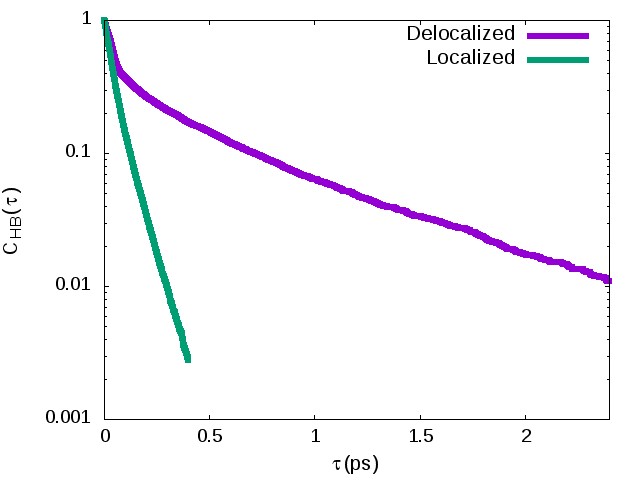
\includegraphics[width=0.4\textwidth]{HB_decay}
\caption{HB decay function for delocalized reference and localized system.} \label{Fig:HBdecay}
\end{figure}

The calculated HB life time for delocalized system is 0.7ps, and for localized system it becomes 0.08ps, indicating that HB are much less stable without covalent interaction. 
 
\textbf{Diple and dielectric constant}
In spite of the ambiguity of the definition of a local dipole moment, we assign each electron to one molecule through the method of maximally localized Wannier centers (MLWC). The resulting dipole distribution in shown in Fig~\ref{Fig:dipoledist}. The average dipole moment of a water molecule is 3.09 Debye for delocalized system and 2.47 Debye for localized system, while for an isolated molecule it is 1.96 Debye. \new Covalent interaction is also partially responsible for the increase of dipole moment from gas to the condensed phase. \old The dielectric constant can be calculated through the fluctuation of the total dipole moment\cite{neumann1983dipole,adams1981theory}:

\bea
\epsilon = 1+\frac{4\pi}{3V k_B T}  (  \langle |\vec{M}|^2 \rangle  - \langle |\vec{M}| \rangle ^2) \label{Eq:dielectric}
\eea

where $V$ is the volume of the system and $\vec{M}$ the total dipole. \new Add results latter.\old

\begin{figure}
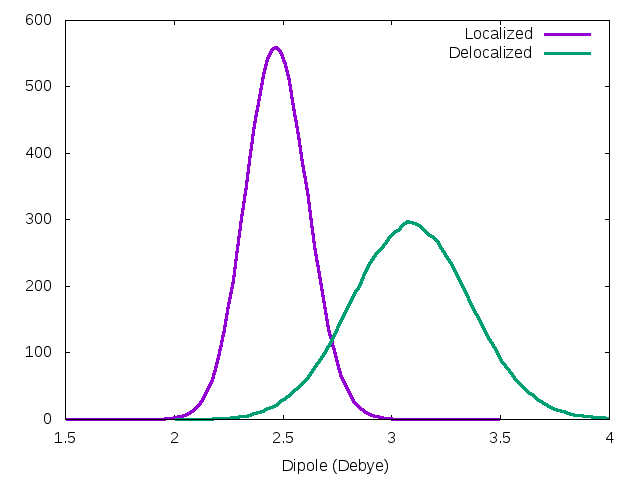
\includegraphics[width=0.4\textwidth]{dipole_dist}
\caption{Dipole distribution of water molecules} \label{Fig:dipoledist}
\end{figure}


\textbf{Infared spectrum.} The infared spectrum for the system is calculated using TRAVIS package \cite{brehm2012travis}. Fig~\ref{Fig:IR} shows the infared(IR) spectrum of the localized and reference systems. For comparison, the IR spectrum of none-interaction water vapor is also shown. The O-H stretch modes(also denoted by $\nu$ band) of the localized system do not show the broadening and shift due to HBs, as in the delocalized system. And now the two peaks for symmetric and asymmetric stretch modes are separate. This implies that these modes are very sensitive to covanlency, and without covanlecy, they are very similar to that of the none-interacting molecules. \new However, the integrated intensity of the $\nu$ band is still $\sim$10 times larger than that of water vapor, which is generally an indication of the existence of HBs. \old Another difference between the localized and delocalized system is the intermolecular modes, they are shifted to lower energy because the intermolecular bonding in localized system is weaker. The bending modes remain roughly the same for localized, delocalized and vapor systems. Since in liquid water, the shift of the centre of $\nu$ band is caused by the coupling between the O-H stretch mode and librations \cite{marechal2006hydrogen}, it then implies that this coupling is mainly through covalent interactions. Furthermore, the narrow spread of $\nu$ band, while the relative position and orientation of neighboring water molecules are larger (as shown in Fig~\ref{Fig:ADF}) also implies that the HBs are now much less sensitive to molecular environment.

\begin{figure}
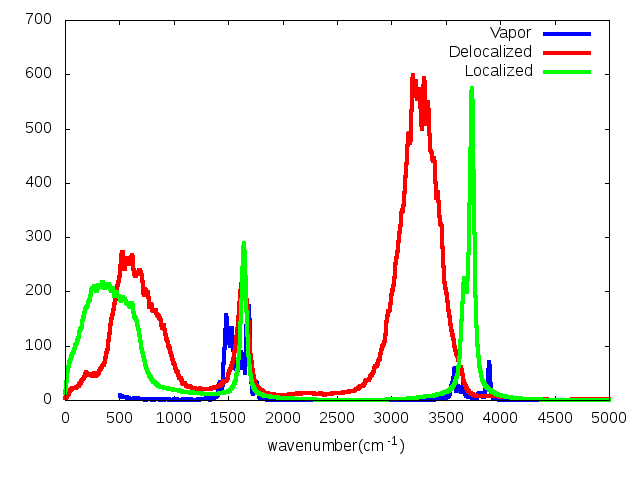
\includegraphics[width=0.4\textwidth]{all_ir}
\caption{IR spectrum. For water vapor, localized and delocalized systems. The low wavenumber part of the spectrum for vapor which corresponds to rotational modes are not shown for simplicity.  The O-H stretch mode ($\sim$3600 cm$^{-1}$) for localized system is very similar to vapor which is none-interaction. And the intermolecular modes ($\sim$500 cm$^{-1}$) moves to the left, indicating the intermolecular bonding is weaker. } \label{Fig:IR}
\end{figure}

\textbf{Diffusion constant and viscosity.} The diffusion constant for a periodic system is known to have strong dependence on the size of the simulation box, due to the interaction of a particle with its periodic images. And the diffusion constant obeys:

\bea
D(\infty) = D(L) + \frac{k_BT\zeta}{6\pi \eta L},
\eea
where $D(L)$ is the diffusion constant for a system of size $L$, $\eta$ is the translational shear viscosity, and $\zeta$ is a constant of 2.837. We calculate the diffusion constant from the mean squre deviation of the molecules, for systems of 64, 125, and 256 molecules, and find the viscosity through the dependence of $D(L)$ on $1/L$, which is shown in Fig~\ref{Fig:dfs}. The result is listed in Tab~\ref{Tab:dfs}. For delocalized reference the calculated viscocity is larger than the experimental value, a consequence of overestimating interaction strength in the XC functional. And it also implies that about 90\% of water's viscosity comes from covalency.

\begin{figure}
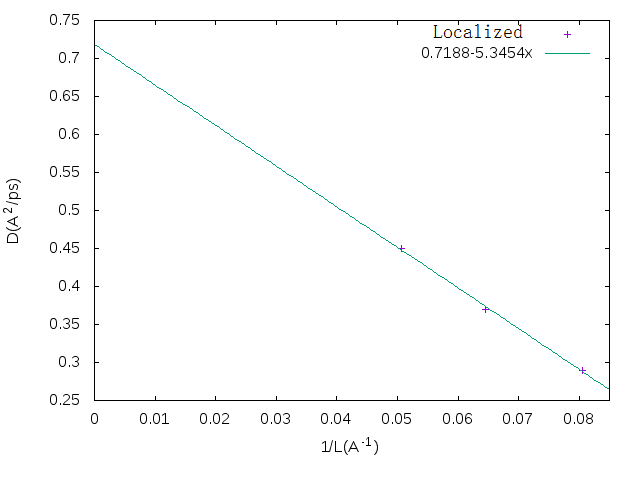
\includegraphics[width=0.4\textwidth]{ALMO_0_msd}
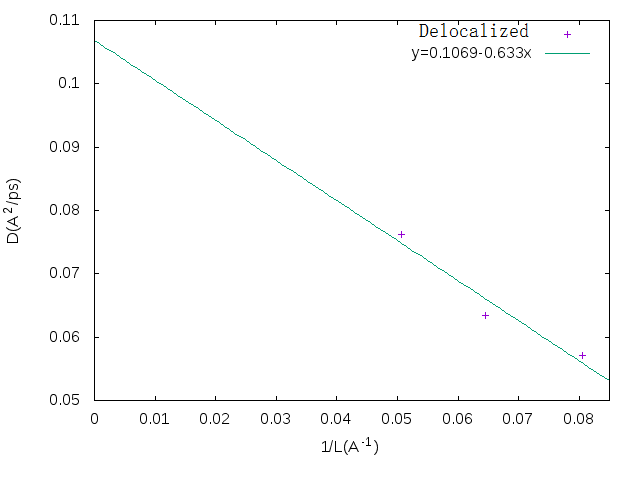
\includegraphics[width=0.4\textwidth]{FULL_SCF_msd}
\caption{Diffusion constant as a function of the system size, for 64, 125 and 256 water molecules. \new error bars?\old }\label{Fig:dfs}
\end{figure} 

\begin{table}
\caption{Viscosity and diffusion constant}\label{Tab:dfs}
\begin{tabular}{l*{6}{c}r}
\hline
               & $D(\mathring{\text{A}}^2/\text{ps})$ & $\eta(\text{Pa}\cdot \text{s})$ \\
\hline
Localized                & 0.7188 & 3.5$\times 10^{-4}$ \\

Delocalized              & 0.1069 & 2.95$\times 10^{-3}$\\

Experimental            & 0.239  & 8.9$\times 10^{-3} $


\end{tabular}

\end{table}


\textbf{Dependence on basis set} It is know that methods that use localized MOs, like ALMO, would overestimate polarization energies in the overlapping regime, especially in the case of large basis set, and lack a meaningfull limit in complete basis set\cite{horn2015polarization}. To ensure that our results are not effect by the basis set, we also run MD simulation with a larger (aug-TZV2P) basis set, and compare the results with the calculation of TZV2P basis set, which is used otherwise in this work. The results are summarized in Fig~\ref{Fig:basis}.

\begin{figure}
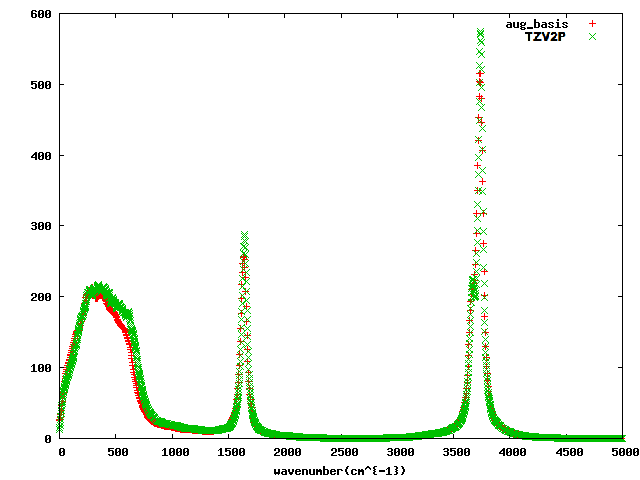
\includegraphics[width=0.35\textwidth]{aug_ir}
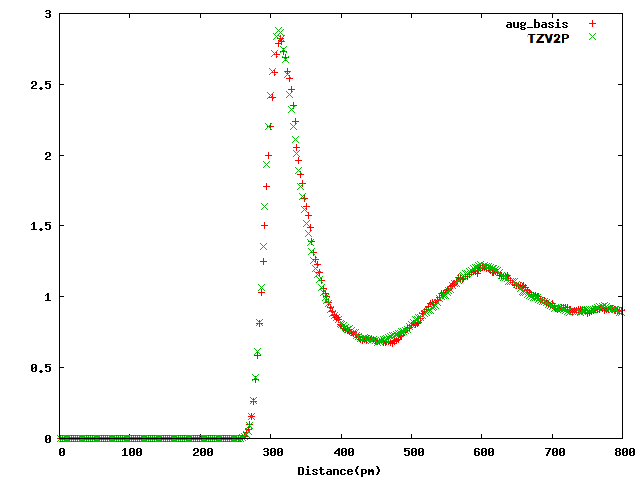
\includegraphics[width=0.35\textwidth]{aug_rdf}
\caption{IR and RDF with aug-TZV2P basis set}\label{Fig:basis}
\end{figure} 

\textbf{Density dependence of localized system} Here we present the calculation of the system at a density of the NPT ensemble at 1atm, which is 0.85g/cm$^3$. The O-O and O-H radial distribution function is shown in Fig~\ref{Fig:rdf_cp}. The position of the peak doesnot move much for the O-O distritution but the peak is more shallow for the low density system. O-H distance tends to be further in the low density system.

\begin{figure}
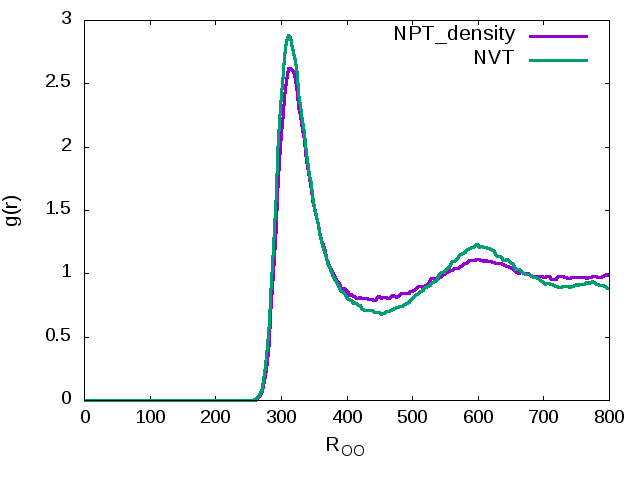
\includegraphics[width=0.45\textwidth]{rdf_NVT_CPDNVT}
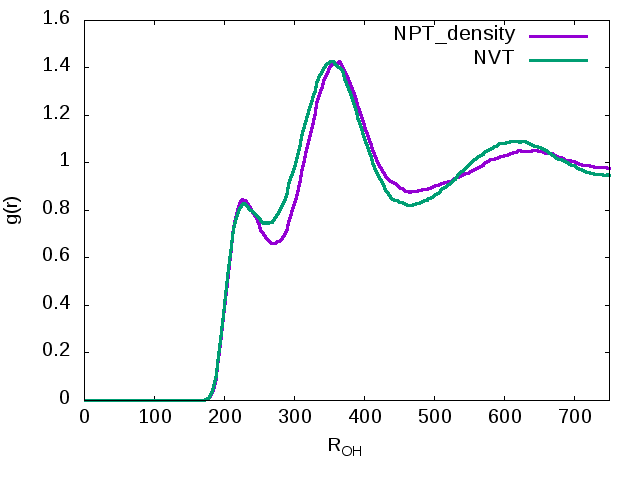
\includegraphics[width=0.45\textwidth]{rdf_OH_NVT_CPDNPT}
\caption{O-O and O-H radial distribution function for the 2 systems. The cutoff for the O-H distance is set to be 2.6$\mathring{A}$.}\label{Fig:rdf_cp}
\end{figure} 

Then angular distribution is shown in Fig~\ref{Fig:adfcp}. Although the interaction for the low density system is weaker, the angular distribution is slightly more ordered. The IR spectrum for the 2 systems are almost identical, as shown in Fig~\ref{Fig:ir_cp}.

\begin{figure}
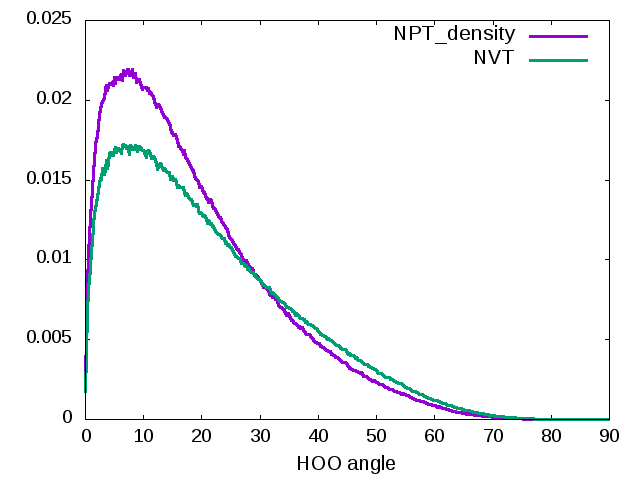
\includegraphics[width=0.45\textwidth]{angular_NVT_NPTCP}
\caption{Angular distribution function for the 2 systems.}\label{Fig:adfcp}
\end{figure} 

\begin{figure}
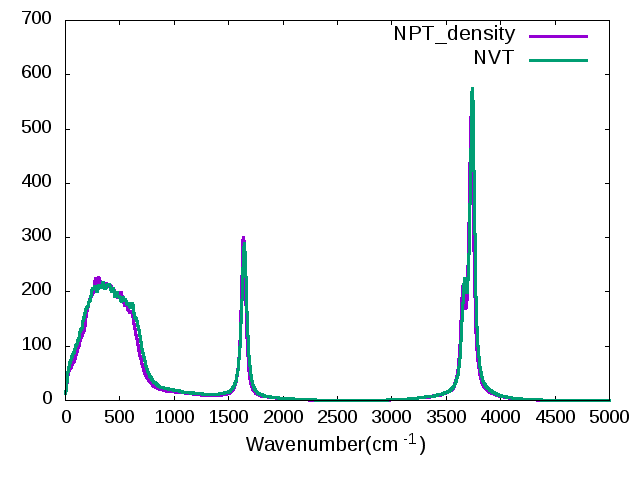
\includegraphics[width=0.45\textwidth]{ir_NVT_NPTCP}
\caption{IR spectrum for the 2 systems.}\label{Fig:ir_cp}
\end{figure} 

\section{Conclusion}
 In this work, we present the effect of the covalent interaction on observable properties of liquid water, and show that although the charge transfer energy only makes up 30\% of the total bonding energy, it plays a dominant rule in some other properties, like the OH stretch mode, viscocity, HB life time. And also significantly changes dipole moment, angular distribution. 
 
 Our result also suggest that classical models that don't take account of covalency only have limit applicability, as they fine-tune the parameters only for certain conditions.
 
 
\textbf{Acknowledgments.} The research was funded by the Natural Sciences and Engineering Research Council of Canada through the Discovery Grant. The authors are grateful to Compute Canada and McGill HPC Centre for computer time.
\bibliography{covalency}
\end{document}
